\documentclass[a4paper, 12pt]{article}

\usepackage[left=2cm, right=2cm, top=2cm]{geometry}
\usepackage{color}
\usepackage{graphicx}
\usepackage{float}

\begin{document}
\pagenumbering{roman}
\title{
		\textbf{Student Name:} Tevin Achong\\
		\textbf{Student ID:} 816000026\\
		\textbf{Course Code:} INFO3606\\
		\textbf{Course Title:} Cloud Computing\\
		\textbf{Assignment:} 1
		\date{February 14, 2020}
}
\maketitle

\newpage
\pagenumbering{arabic}

\begin{center}
	\textbf{Question 1}\\
\end{center}

\textbf{What is cloud?}\\
Cloud refers to servers that are accessed over the Internet, and the software and databases that run on those servers. Cloud servers are located in data centers all over the world.\\

\textbf{What is cloud computing?}\\
Cloud computing is a model for enabling ubiquitous, convenient, on-demand network access to a shared pool of configurable computing resources (e.g. networks, servers, storage, applications, and services) that can be rapidly provisioned and released with minimal management effort or service provider interaction. This cloud model is comprised of five essential characteristics, three service models, and four deployment models.\\

\textbf{Explain the cloud cost model.}\\
Cloud service providers typically use the \textbf{Measured Service and Pay-as-Per-Use Pricing Model:}
\begin{itemize}
\item
The cloud environment provides automatic-metering capability to measure the resources utilized by consumers, which is done in a transparent manner for both providers and users.
\item
According to the service measured, consumers will be billed.
\item
As for what is measured a provider will charge a consumer only for the IT resources actually used and/or for the time frame during which the resources were used.
\item
Similar to how the public pays for different utilities, such as gas, electricity,  etc., cloud consumers are charged for their exact use of resources.
\item
There are typically two pricing schemes provided in the cloud environment: \textit{subscription-based pricing} (like a monthly bill for the service acquired) or \textit{pay-as-per-use pricing}, as outlined in the points above.
\end{itemize}

\newpage
\begin{center}
	\textbf{Question 2}\\
\end{center}

\textbf{What are the cloud service models?}\\

The types of cloud service models are:
\begin{itemize}
\item[i.]
IaaS (Infrastructure as a Service)
\item[ii.]
PaaS (Platform as a Service)
\item[iii.]
SaaS (Software as a Service)
\end{itemize}

\textbf{Describe what are IaaS, PaaS and SaaS and the relationships among them.}\\

\underline{IaaS}:\\
The capability provided to the consumer is to provision processing, storage, networks, and other fundamental  computing resources where the consumer is able to deploy and run arbitrary software, which can include operating systems and applications. The consumer does not manage or control the underlying cloud infrastructure but has control over operating systems, storage, and deployed applications; and possibly limited control of select networking components (e.g. host firewalls).
\begin{itemize}
\item
IaaS allows distributed virtualized computational resources, such as servers, storage devices, network devices, and virtual machines, to be shared.
\item
The IaaS environment can be likened to an on-premises infrastructure.
\item
It can be seen that in an on-premises facility control entirely lies with the enterprise, whereas in an IaaS service model the provider completely controls and maintains the physical infrastructure.
\item
Cloud users can control the virtual machines and other platforms on top of the physical infrastructure.
\item
IaaS providers offer (i) servers, (ii) storage, (iii) networks, (iv) hypervisors, and (v) virtual machines to users.
\item
On top of the virtual machine users install their required guest operating system, middleware, runtime, data, and applications according to their needs:
\begin{itemize}
\item
IaaS cloud providers offer their resources on-demand from their large pools of physical infrastructure. Very often the infrastructure is distributed across different geographical locations. IaaS providers employ cloud orchestration technology using software such as OpenStack, Apache CloudStack, or Open Nebula to create and manage virtual machines (VMs). Cloud orchestration involves carrying out automatic resource provisioning according to dynamic needs. It decides the most appropriate physical host to assign to VMs, performs VM migration from one host to another whenever required, allocates storage volumes to VMs, and provides usage information for billing.
\item
This kind of service is suitable for organizations that have difficulty funding the basic infrastructure to run their businesses. IaaS is the right choice for organizations looking for high levels of customization for their infrastructure.
\item
IaaS  normally  requires  a  high  degree  of  technical  proficiency  to  configure  the infrastructure  acquired  from  cloud  providers.  Hence  IaaS  is  more  suitable  for enterprises  with  a  highly  skilled  set  of  developers,network  administrators,  and database administrators who can work as a team to build applications from scratch, manage network traffic and storage traffic, and maintain and scale up or scale out requirements according to the needs of enterprise applications.
\item
Responsibilities  are  shared  by  both  IaaS  providers  and  consumers.  With  an  IaaS model providers gain control over actual physical hardware resources. Users have control only overresources that are above the virtual machine. In the case of an on-premises infrastructure complete control, responsibility, and management lies with the  owners.  Among  the  most  popular  IaaS  providers  are  Amazon  Web  Services (AWS),  Cisco  Metapod,  Microsoft  Azure,  Google  Compute  Engine  (GCE),  and Joyent.
\end{itemize}
\end{itemize}

\underline{PaaS}:\\
The capability provided to the consumer is to deploy onto the cloud infrastructure consumer created or acquired applications created using programming languages, libraries, services, and tools supported by the provider. The consumer does not manager or control the underlying cloud infrastructure including network, servers, operating systems, or storage, but has control over the deployed applications and possibly configuration settings for the application-hosting environment.
\begin{itemize}
\item
Platform  as  a  Service  (PaaS)  providers offer  users  both  the  hardware  structure  and software platform needed for applications development. 
\item
In general, PaaS providers offer both the underlying hardware infrastructureand softwareplatform such as web servers, application servers, database servers, and a programming environment (e.g., J2EE, .Net, or Python).
\begin{itemize}
\item
Developers can use PaaS as a platform or framework to develop and customize their applications.
\item
PaaS makesthe development, testing, and deployment of applications quick and cheaper.
\item
PaaS models provide benefits such as increased developer productivity and short time to market for applications.
\end{itemize}
\item
However, in the PaaS model users gain control only over applications they install on the  platform  and  data.  They  have  no  control  over  the  underlying  hardware  and platform,  which  are  completely  managed  by  PaaS  providers.
\item
Popular  PaaS  providers  include  Google  App  Engine,  Microsoft  Azure,  and  RedHat OpenShift.
\item
Google  App  Engine  and  RedHat  OpenShift  provide  a  complete  platform  for  the development  of  distributed  webapplications  based  on  an  open-source  environment, whereas  Microsoft  Azure  offers  a  platform  for  both  Windows-based  and  open-source tools, such as .Net, Python, Ruby, andPHP, for applications.
\end{itemize}

\underline{SaaS}: The capability provided to the customer is to use the provider's applications running on a cloud infrastructure. The applications are accessible from various client devices through either a thin client interface, such as a web browser (e.g. web-based email), or a program interface. The consumer does not manage or control the underlying cloud infrastructure including network, servers, operating systems, storage, or even individual application capabilities, with the possible exception of limited user-specific applicatoin configuration settings.
\begin{itemize}
\item
Software  as  a  Service  (SaaS)  allows  cloud  service  providers  to  offer  completely developed applications to users over the internet on a subscription basis. 
\item
Users can simply log in and use applications completely provided by SaaS providers and run on the providers’ infrastructures.
\item
In this model users have no control at all over anything.
\item
All layers are under the control of SaaS providers.
\end{itemize}

\textit{All the service models have the fundamental characteristics of cloud computing, elasticity, scalability, on-demand computing, multi-tenancy, metering service, and pay-per-use pricing model. Similarly, they have the same limitations, such as data integrity, security, and vendor lock-in.}

\newpage
\begin{center}
\textbf{Question 3}\\
\end{center}
\textbf{What are the cloud components?}\\
The three major cloud components are:
\begin{itemize}
\item[i.]
The front end
\item[ii.]
The network
\item[iii.]
The backend / the cloud
\end{itemize}

\textbf{Please describe the cloud architecture based on these components.}\\
The aforementioned components make up the cloud computing architecture.\\

\underline{Front End:}
\begin{itemize}
\item
The front-end layer of the cloud refers to the user layer.
\item
Typical cloud users are individuals, enterprises, employees of enterprises, employees on the move, mobile users, laptop users, users having any kind of connected device etc.
\item
Cloud service providers provide APIs and interfaces for users themselves to access the required service through a web portal.
\item
Users access the APIs over the internet and consume the required service.
\end{itemize}

\underline{Network:}
\begin{itemize}
\item
Network refers to the broad backbone infrastructure through which cloud service providers offer their services to users.
\item
The internet is the core network infrastructure that makes cloud computing feasible.
\item
Services are delivered via the internet.
\item
Typically, users can access public clouds directly via the internet and private clouds via a secure VPN over the internet.
\end{itemize}

\underline{Back End:}
\begin{itemize}
\item
The back-end layer forms the cloud.
\item
It consists of six different layers:
\begin{itemize}
\item[(i)]
Physical layer
\item[(ii)]
Virtualization layer
\item[(iii)]
Layer of cloud services
\item[(iv)]
Scheduling, provisioning, and pricing layer
\item[(v)]
Security
\item[(vi)]
Management
\end{itemize}
\end{itemize}

\newpage
\begin{itemize}
\item[(i)]
\textit{Physical layer}
\begin{itemize}
\item
The core component of the cloud is the physical infrastructure.
\item
The physical infrastructure includes bare metal hardware, servers, CPUs, storage devices, network devices, any other network-related hardware, and memory.
\item
The physical infrastructure is not to be found at a single location, rather it is distributed across different geographical locations.
\item
Resources are heterogeneous in nature. 
\end{itemize}

\item[(ii)]
\textit{Virtualization layer}
\begin{itemize}
\item
The virtualization layer is responsible for considering theoretically all the heterogeneity and physical distribution of the underlying hardware and generate a single, logical view for the entire physical layer of the cloud.
\item
This is achieved with software called Virtual Machine Monitor (VMM) or hypervisor.
\item
Hypervisor combines all the physical hardware and produces a unified global and logical view of resources that will then be allocated to multiple tenants according to their dynamic demands.
\end{itemize}

\item[(iii)]
\textit{Layers of cloud services}
\begin{itemize}
\item
Cloud service providers offer different kinds of services.
\item
The major service classes are Infrastructure as a Service (IaaS), Platform as a Service (PaaS), and Software as a Service (SaaS).
\item
A cloud service provider generally provides only one kind of service.
\item
However, a service provider may provide more than one service offering. For example, Azure initially provided only PaaS, but later it started providing both PaaS and even some IaaS services. 
\item
These services are offered on top of the virtualization layer.

\item
\textit{\underline{Infrastructure as a Service}}
\begin{itemize}
\item
Infrastructure service providers typically offer hardware, storage devices, servers, network components, and other hardware to users to support their operations.
\item
Infrastructure service providers are responsible for housing, operating, and maintaining the hardware for clients.
\end{itemize}

\item
\textit{\underline{Platform as a Service}}
\begin{itemize}
\item
Platform providers offer a cloud-based computing environment to design, develop, execute, and manage applications.
\item
Platform providers typically provide development platforms, middleware, operating systems, programming languages, libraries, runtime environments, application servers, database management servers, load balancers, business analytics services, mobile backend services, integration brokers, business process management systems, rules engines, event processors, and other software tools.
\item
PaaS providers are responsible for installation, configuration, operation, licensing, upgradation of software tools, and maintenance of tools.
\item
PaaS providers help developers to concentrate only on developing code of concern to them and hence to relieve them of the abovementioned common services.
\end{itemize}

\item
\textit{\underline{Software as a Service}}
\begin{itemize}
\item
Software as a Service provides software applications for consumer use over the internet on demand.
\item
Users can subscribe to software applications from SaaS providers with the help of their APIs over the internet.
\end{itemize}

\end{itemize}

\item[(iv)]
\textit{Scheduling, provisioning, and other services}
\begin{itemize}
\item
Various management and orchestration services are needed to be able to manage the cloud environment.
\item
Cloud orchestration and management are essential processes that take place within the cloud. A cloud orchestrator automates and orchestrates:
\begin{itemize}
\item
a scheduling component to schedule resources to different tenants;
\item
a provisioning component that provides scheduled resources;
\item
monitoring components that monitor the cloud environment;
\item
metering services that meter the resources provided; and
\item
a pricing component that bills the consumer according to a subscription-based or use-based model.
\end{itemize}
\end{itemize}

\item[(v)]
\textbf{\textit{Security}}
\begin{itemize}
\item
Security in cloud computing is a responsibility shared among cloud service providers and cloud users.
\item
In the case of IaaS, for example, providers take on the responsibility of providing security for their physical infrastructure and consumers take on the responsibility of providing security to a guest operating system (OS), platform, applications, and data that they deploy on the infrastructure consumed.
\end{itemize}

\item[(vi)]
\textbf{\textit{Management}}
\begin{itemize}
\item
Since cloud computing environment is complex, cloud service providers user various tools to manage, automate, and orchestrate cloud operations and business services.
\item
Cloud Management Platform (CMP) tools, cloud automation tools, cloud orchestration tools, cloud brokerage tools, cloud monitoring tools, cloud security tools, etc. are typically used to manage and optimize the cloud.
\end{itemize}

\end{itemize}


\newpage
\begin{center}
\textbf{Question 4}\\
\end{center}
\textbf{What is virtualisation?}
\begin{itemize}
\item
In the cloud infrastructure, there are three kinds of services, Infrastructure as a Service, Platform as a Service, and Software as a Service.
\item
IaaS providers theoretically offer any number of of hardware resources, such as servers and storage devices, for use according to the dynamic demands of users.
\item
PaaS providers offer almost all kinds of platforms along with infrastructure to users wanting to deploy their applications without worrying about the resources needed for load balancing, scalability, performance, etc.
\item
SaaS providers offer completely developed cloud-deployed software applications that users can consume on a subscription basis.
\item
These services are provided simultaneously to many consumers.
\item
The huge resources of cloud service providers are shared among multiple users.
\item
\textit{\textbf{Virtualization} is the the technology that enables this kind of sharing of resources among multiple users simultaneously and enables each user to have varying demands.}
\item
Since cloud service providers offer servers, storage, and networks the concept of virtualization is applied at different levels (such as servers, storage, networks, memory, data, applications, and desktops) so as to yield virtualized storage, virtualized networks, virtualized memory, virtualized data, virtualized applications, virtualized desktops etc.
\item
Hence, virtualization is key to the implementation of cloud computing.
\item
In a nutshell, \textbf{\textit{virtualization is the creation of virtual resources, such as servers, storage devices, networks, adn desktops, by abstracting the heterogeneity in hardware. This is being pursued by cloud service providers to effectively use their computational resources and maximize their profits.}}
\end{itemize}


\textbf{Describe different layers of virtualisation.}\\
\underline{Server Virtualization}
\begin{itemize}
\item
Server virtualization provides the capability to create many virtual servers on top of the real physical server by separating and abstracting the real server (i.e., a machine with CPU, RAM, hard disk etc.) from the rest of the system. 
\item
The primary objective of server virtualization is to increase resource utilization by partitioning a single physical server into many virtual servers where each virtual server has its own operating system and applications.
\item
Moreover, each virtual server is unaware of the presence of other servers. Each virtual machine is logically separated from other virtual servers.
\item
Conventionally, each server is tied to a particular operating system and, typically, a particular application is deployed in a server.
\end{itemize}

\underline{Desktop Virtualization}
\begin{itemize}
\item
In desktop virtualization the hardware, operating system, applications, data, and user profile of a real desktop can be abstracted from a client machine to a remote server.
\item
After desktop virtualization, a user will work with a virtual desktop in a cloud server.
\item
When a client accesses a desktop all applications and corresponding data are accessed from a central server.
\end{itemize}

\underline{Data Virtualization}
\begin{itemize}
\item
Data virtualization is the concept of aggregating data from heterogeneous data sources at different locations into single items of data and logical data that can be accessed easily by applications.
\item
Data virtualization facilitates data access, data integration, and data management by providing a single data management model.
\item
The primary advantage is that data consumers can retrieve and manipulate data from one or more data sources without knowing the technical details of data storage such as API, access language, storage structure, or its format or location.
\item
Data virtualization facilitates real-time access to data. Data virtualization reduces data errors and helps to combine the results of data sets from multiple data sources so as to produce \textit{federated data} and make such data available to users.
\end{itemize}

\underline{Application Virtualization}\\
\begin{itemize}
\item
In application virtualization a given application in a particular operating system is made to execute in a virtual way on any operating system.
\item
Application virtualization abstracts applications from underlying operating systems.
\item
Deploying an application in traditional systems means packaging parts of the application and installing the application according to the requirements of the target operating system and machine.
\item
The application virtualization layer in the cloud environment fools applications into getting deployed in any virtual guest operating system.
\end{itemize}

\underline{Memory virtualization}
\begin{itemize}
\item
The physical memory across different servers is aggregrated into a single large primary memory that is accessible by applications deployed in virtual machines.
\item
In general, there are three memory addresses: a machine address that represents the actual physical address sent on the bus to memory, a guest physical address that represents the virtual address of memory as seen by the guest OS, and a guest virtual address that represents the virtual address as seen by the guest application. 
\item
As memory is very closely involved with compute logic, enterprises need to add memory to achieve higher performance of applications. However, adding memory is very expensive.
\item
Memory virtualization helps to share existing memory across many servers as a single larger memory. Hence it helps in achieving higher performance at lower cost.
\end{itemize}

\underline{Network virtualization}
\begin{itemize}
\item
Network virtualization refers to the creation of more than one logical and virtual network that work simultaneously and share the same single physical network.
\item
These logical networks are also called \textit{network overlays}. Network virtualization allows users to create their network with their own topology, routing, and other application-specific requirements including resource management.
\item
The most important aspect of network virtualization is that it avoids some of the critical issues associated with the current internet: Internet Protocol (IP) ossification, issues with end-to-end quality of service, and lock-in of customers with their internet service providers.
\item
Network virtualization handles the above issues, provides high throughput for data transmission, and delivers control over end-to-end quality of service.
\item
The virtualization layer helps to create virtual networks according to the requirements of the top layer of VMs and their applications.
\item
Hence, any application can configure its required topology, routing, and the other network stuff with virtual networks instantly and gain network connectivity.
\item
Network virtualization restricts the movement of data and information across networks and enhances security.
\item
The most important aspect is that each virtual network is isolated and independent of other networks.
\end{itemize}

\underline{Storage virtualization}
\begin{itemize}
\item
Storage virtualization is the concept of abstracting or hiding heterogeneity among different storage devices from the applications that manage them.
\item
Different techniques may be used to get the different physical storage devices to aggregrate in a pool of logical storage that can be accessed and managed in a unified way from a centralized console.
\item
In conventional storage management with no storage virtualization, storage management has to deal with the varying characteristics of different storage devices as well as vendor-specific features.
\item
Conventionally, storage management has dealt with each device as a discrete unit.
\item
The primary difficulty with conventional storage is how to deal with heterogeneous storage devices. Another difficulty is that the devices are manufactured by different vendors.
\item
In \textit{virtualized storage}, various devices are aggregrated into a single pool of logical storage by the storage virtualization layer.
\item
This layer hides the heterogeneity of devices and provides a uniform way of managing them.
\end{itemize}

\textbf{What is hypervisor?}\\
A hypervisor, also called Virtual Machine Monitor (VMM), is essentially computer software, hardware, or firmware that creates and runs virtual machines. It is located in the virtualization layer of the back-end of the cloud architecture.\\

\textbf{What does a hypervisor do?}\\
The virtualization layer is responsible for considering theoretically all the heterogeneity and physical distribution of the underlying hardware and generate a single, logical view for the entire physical layer of the cloud. \textbf{This is achieved with software called \underline{hypervisor}.} Hypervisor combines all the physical hardware and produces a unified global and logical view of resources that will then be allocated to multiple tenants according to their dynamic needs.

\newpage
\begin{center}
\textbf{Question 5}\\
\end{center}
\textbf{Describe how technological drivers fit into different layers of the cloud architecture.}\\
Cloud computing has developed very rapidly as a result of various technological drivers. These include:
\begin{itemize}
\item
Open source tools and APIs
\item
Software defined security
\item
Virtualization and containerization
\item
Multi-core technology
\item
WAN, internet, SOA, Web 2.0
\item
Parallel programming
\item
Grid and utility computing
\item
Software defined networking
\item
MSA, DevOps, Agile
\end{itemize}

Figure 1 below depicts how each of these fit into different layers of the cloud architecture.\\

\begin{figure}[H]
	\centering
	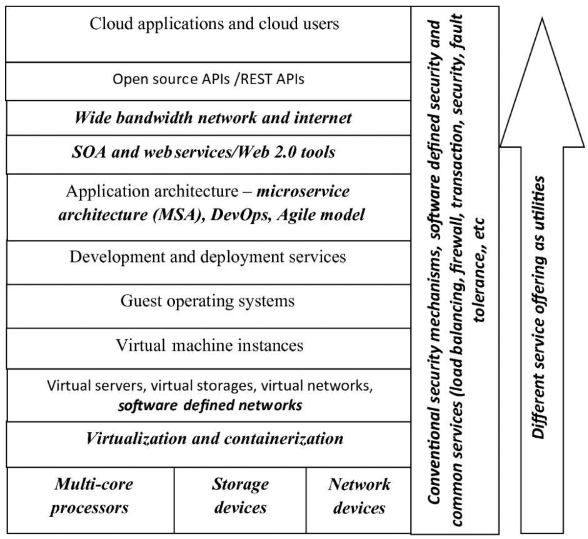
\includegraphics[width=\linewidth]{technological_drivers.png}
  	\caption{How the different technological drivers fit into different layers of the cloud architecture}
	\label{fig:4-waycache}
\end{figure}

\begin{itemize}
\item
In the cloud infrastructure there are three kinds of services: Infrastructure as a Service, Platform as a Service, and Software as a Service. IaaS providers theoretically offer any number of hardware resources, such as servers, storage devices, and networks, for use according to the dynamic demands of users.
\item
PaaS providers offer almost all kinds of platforms along with infrastructure to users wanting to deploy their applications without worrying about the resources needed for load balancing, scalability, performance, etc.
\item
Similarly, SaaS providers offer completely developed cloud-deployed software applications that users can consume on a subscription basis.
\item
These services are provided simultaneously to many consumers.
\item
The huge resources of cloud service providers are shared among multiple users.
\item
Virtualization is the technology that enables this kind of sharing of resources among multiple users simultaneously and enables each user to have varying demands.
\item
Since cloud service providers offer servers, storage, and networks the concept of virtualization is applied at different levels (such as servers, storage, networks, memory, data, applications, and desktops) so as to yield virtualized servers, virtualized storage, virtualized networks, virtualized data, virtualized applications, virtualized desktops, etc.
\item
Hence virtualization is key to the implementation of cloud computing.
\item
Along with virtualization another technique called \textit{containerization} has recently appeared on the scene.
\item
Containerization is more efficient than virtualization when it comes to the efficient utilization of resources.
\item
Recent advances in hardware technologies have led to the \textit{production of multi-core processors} at mass scale.
\item
Corresponding with advances in hardware, software programming models have been developed to support \textit{parallel programming} and simultaneous execution of programs.
\item
In addition, since cloud computing has its roots in \textit{grid computing} and \textit{utility computing}, both of which cast light on how computing resources could be shared similar to domestic utilities using a \textit{pay-per-use pricing model}, it too can be used in like manner.
\item
Wrapping technologies (such as service-oriented architecture) form other major pillars supporting cloud computing.
\item
The internet, IP, WAN, MPLS, WAN, software-defined networks, and software-defined security have significantly influenced the growth of cloud computing.
\end{itemize}

%\underline{Multi-core Technology and Parallel Programming Models}
%\begin{itemize}
%\item
%The cloud computing environment is primarily built on top of multi-core technology.
%\item
%The vendors of microprocessors, such as Intel, AMD, IBM, and Sun, produce multi-core processors.
%\item
%For example, \textit{Intel dual-core processors} are integrated in personal computers and laptops. Recently, Intel introduced \textit{core technology} and \textit{64-core architecture}.
%\end{itemize}

\end{document}
